\chapter{Arduino}\label{analysis:arduino}
Arduino was created by the Interaction Design Institute Ivrea (Italy), by Massimo Banzi and David Cuartielles. They were looking for an easy and cheap way for students, who study design, to integrate micro controllers into their projects\cite{arduino:hist}. Both the board and the programming language was based on the works of Hernando Barragán, one of Massimo Banzi master thesis students \cite{Wiring:thesis}

\section{The hardware components}
Arduino is a single-board micro-controller, see figure \ref{fig:Arduino}.
A board consists of open source hardware, which is designed around an 8-bit Atmel AVR micro-controller. Arduino boards varies in sizes. Arduino Uno board for example, has a max width of 2.1'' (5,33cm) and a length of 2.7'' (6,86cm).  \\

\par
\raisebox{-.5\height}{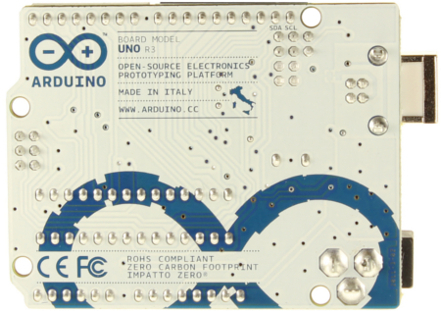
\includegraphics[width=6.5cm]{billeder/ArduinoUno_R3_Back_450px.jpg}}
\hfill
\raisebox{-.5\height}{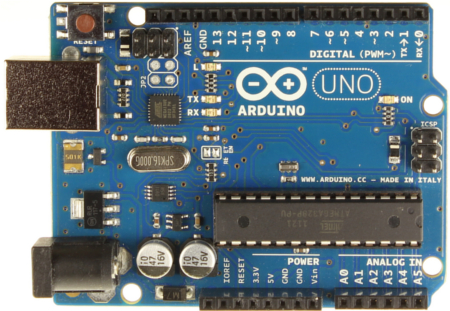
\includegraphics[width=6.5cm]{billeder/ArduinoUno_R3_Front_450px.jpg}}
\begin{figure}[H]
\caption{Picture of back- and fronside of the Arduino board \cite{Arduino_board_pics}}
\label{fig:Arduino}
\end{figure}
\par

The board provides some input and output possibilities. However these vary depending on the board, though most have 14 digital I/O and 6 analog inputs. The I/O functions are placed on top of the board, are freely accessible, and consist of 0.1'' female headers. Besides the I/O there is also a Power connector, which almost in all cases require 5 volt DC. There is a USB connection on the board, so that processing data to the micro-controller is possible, though it is shown as a virtual com-port on the connected computer. However, on older boards, instead of the USB connection, a RS232 were used for serial communication. 

On the board there is a LED diode which is connected to the digital pin 13. When this diode is set to ``HIGH'' it will be turned on, and if its value is ``LOW'' it turns off. Besides the LED diode, there is also a reset button. If the button is pressed the micro-controller is reset. 

Arduino board gain extra features through shields. Shields is a ``board'', or rather an expansion board, which is plugged onto the Arduino board. This provides Arduino boards with the possibilities to control extra components for example motors, sensors and LCD displays.

